%************************************************
\chapter{Conclusion}\label{ch:conclusion}
%************************************************
\section{Summary of Discoveries}

The goal of this dissertation was to make fundamental discoveries that will inform the control of smart stormwater systems, specifically focusing on statistical learning approaches that can be used to generate safe and reliable control algorithms.
To that end, a number of fundamental discoveries were made in each chapter: 

\begin{itemize}
	\item \textbf{Chapter 2:} I have discovered that by controlling the hydrological responses in the stormwater basins the rate of removal of specific nutrients can be targeted. In this chapter I also develop a modular framework for simulating smart stormwater systems.
	\item \textbf{Chapter 3:} I have discovered that the response of the stormwater systems can be precisely shaped by relying on the sensor data. I demonstrate this by shaping the response of 00 $km^2$ watershed by coodinating the control actions of two assets to realize a watershed scale control objective.
	\item \textbf{Chapter 4:} I have demonstrated that deep reinforcement learning methods though show promise in the controlling stormwater systems, their performance is continent on a lot of factors 
	\item \textbf{Chapter 5:}
	\item \textbf{Chapter 6:}
\end{itemize}
\section{Future Directions}

\begin{figure}[H]
	\centering
	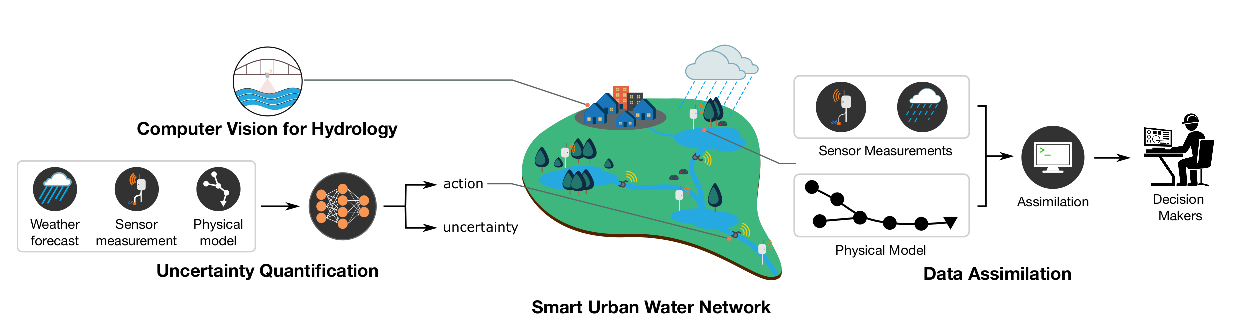
\includegraphics[width=\textwidth]{gfx/rs_final.eps}
\end{figure}

\noindent \textbf{Computer vision for hydrological monitoring}\\
Dynamics that govern the flow of water in urban systems are highly complex and are modeled using a parametrized version of simplified Navier-Stokes equations.
These model parameters require frequent calibration and validation to ensure that they accurately represent the physical system.
Given the steep financial investment and technical expertise required for maintaining a sensor network of flow and depth sensors, high resolution data necessary for calibrating these models is rarely available.
Recent advances in electronics have made large scale deployment of cameras and edge processing financially viable, and computer vision methods have matured to a point where they can be reliably used for detection, segmentation, and tracking.
By adopting these methods for monitoring hydrological phenomenon, a camera can be repurposed to act as a flow, water level, and rainfall sensor.
Thus, creating an affordable alternative for acquiring high resolution on-the-ground measurements. 
City of Chicago and Chicago river are ideal for prototyping this technology.
Cameras from the array of things sensor nodes in Chicago, and the network of flow and rainfall gauges maintained by the  United States Geological Survey and the City of Chicago, provide reliable sources of data for the development and validation of these methods.
%Combining the cameras from array of things sensor nodes in the city with the United States Geological Survey and the Metropolitan City of Chicago's network of flow and rainfall gauges, we have reliable sources of data to develop and validate these methods.
As a deliverable from this project, I hope to create a standalone library that can be integrated with the existing open-source sensing platforms like waggle and open-storm to monitor hydrological phenomenon using image data. 
% Summary: Chicago would be an ideal location for prototyping this technology. Using the camera feeds from the array of things nodes and the flows measurements from the usgs sensors in the river. Particle tacking and feature detection would be a good starting point for this effort. A project deliverable I hope to create an stand alone edge deployable module that can be integrated with the measurements platforms like waggle or open-storm.

\

\noindent \textbf{Data assimilation for reliable urban water models}\\
As the density of sensors in the urban water networks increases, it presents an opportunity for us to go beyond the use of sensor measurements for calibration, and create an integrated approach where this data is assimilated into the physical models to accurately represent the state of the water network for operational decision making.
EPA-SWMM, an open-source hydraulic solver, is extensively used by water utilities and researchers across the world for modeling urban water networks. 
I would like to extend the functionality of EPA-SWMM's core simulation engine to incorporate sensor measurements as boundary conditions, which can then be used to nudge the model estimates.
As a deliverable from this effort, I envision an open-source python library that acts as an add-on module to EPA-SWMM, enabling users to retain existing workflows, and seamlessly shift between the classical SWMM simulation engine and the modified one. 
This library would also act as an interface for the users to define the various sensors streams and the corresponding filtering modules that they would want to integrate with their workflow.

\

\noindent \textbf{Uncertainty quantification for the control of urban water networks}\\
As the urban water infrastructure models become reliable, they can be leveraged to develop coordinated control strategies that enable infrastructure to reprogram itself in real-time to tackle dynamic weather conditions.
A major barrier for the adoption of such an approach, is the uncertainty associated with the underlying model, sensors measurements, and weather forecasts that dictates the actions taken by the control algorithm.
Quantifying these uncertainties will enable the decision makers to weigh the risks and rewards associated with control strategies and pick the one that benefits both the public and environment.
Bayesian optimization, with Gaussian Processes at its core, is an effective approach for searching though the solution space to identify an optimal control strategy and estimate the uncertainty associated with the identified strategy.
But the non-parametric nature of the Gaussian Processes limits the scalability of this approach.
By replacing the Gaussian Processes with Bayesian Neural Networks and Deep Gaussian processes, I want to extend the Bayesian Optimization approach for quantifying the uncertainties in large scale urban water networks. 
As a deliverable, I hope to create a open-source python toolbox that interfaces with the existing SWMM models to help the decision makers identify a control strategy and its associated uncertainty, for achieving a desired behavior in the urban water network.

\

% Summary Tie all of it together and speak to the potential of applied computational tools in water.
\noindent Industries like autonomous driving have completely embraced wireless sensing and machine learning. 
But its adoption in civil engineering has been limited to research.
Given the number of such systems in United States, even a marginal performance improvement of 5\% can have a significant positive impact on the environment.
There is a huge disparity between the current state-of-art in urban water systems and the possibilities enabled by the adoption of these technologies.
This huge potential for improvement, at a margin of the cost of traditional solutions, has been a strong motivator for my research.
Urban water systems are an essential part of the city's infrastructure, and there are significant socio-technical challenges that have to addressed before these autonomous water systems become commonplace. 
Developing open source tools that are accessible to researches and stakeholders, from both engineering, social sciences, and policy making, enables us to ease the transition of these technologies into practice.

